\question{Диод на высоких частотах. Особенности движения и траектории электронов
  в плоском диоде на высоких частотах}

Первые электроны, эмитируемые с катода, движутся без влияния сил
пространственного заряда. Уравнение движения имеет вид:
\[
  m\ddot{z} = e\frac{U_a}{d}; \qquad
    m\ddot{z} = \frac{e}{d} \big( U_{a0}\sin\omega t - U_0 \big), \ \
    \big( U_0 < 0 \big).
\]

Эмиссия с катода начинается в момент времени, определяемый по формуле
\eqref{eq26t0}. Из нее следует, что \( U_0 = U_{a0}\sin\omega t_0 \). Тогда
уравнение движения преобразуется к виду
\[
  m\ddot{z} = \frac{e}{d}U_{a0} \bigl( \sin\omega_t - \sin\omega t_0 \big).
\]

Интегрируем, получаем:
\[
  \dot{z} = \frac{e}{md\omega}U_{a0} \big( -\cos\omega t -
    \omega t\sin\omega t_0 \big) + C_1.
\]

Поскольку мы пренебрегаем начальной скоростью электронов, то
\[
  \dot{z}\Big|_{t = t_0} = 0\colon \quad
    C_1 = \frac{e}{md\omega}U_{a0} \bigl(\cos\omega t_0 +
    \omega t_0\sin\omega t_0\big).
\]

Тогда \( \dot{z} \):
\[
  \dot{z} = \frac{eU_{a0}}{md\omega}\Bigl[ \cos\omega t_0 - \cos\omega t +
    \omega \big( t_0 - t \big) \sin\omega t_0 \Big].
\]

Проинтегрируем это выражение. Обозначая \( \alpha = md\omega^2 / (eU_{a0}) \),
получим следующее:
\[
  \alpha z = \omega t\cos\omega t_0 - \sin\omega t + \omega t \left( \omega t_0
    - \frac{\omega t}{2} \right) \sin\omega t_0 + C_2.
\]

Примем положение катода за 0:
\[
  z\Big|_{t = t_0} = 0\colon \quad
    C_2 = \frac{1}{\alpha} \left[ \left( 1 - \frac{\omega^2 t_0^2}{2} \right)
    \sin\omega t_0 - \omega t_0 \cos\omega t_0 \right].
\]

В итоге имеем выражение:
\begin{equation}
  \alpha z = \bigl( \omega t - \omega t_0 \big)\bigl[ \cos\omega t_0 +
    \omega t_0 \sin\omega t_0 \big] - \sin\omega t + \sin\omega t_0 + \left(
    \frac{\omega^2 t_0^2}{2} - \frac{\omega^2 t^2}{2} \right) \sin\omega t_0.
  \label{eq27az}
\end{equation}

Последующие электроны движутся под действием сил пространственного заряда, что
эквивалентно изменению напряжения на аноде, поэтому \( U_a' = U_a - U_0' \), где
\( \displaystyle
  U_0' = \frac{\alpha}{\Ez} \int\limits_0^d \abs{\rho}\,dz
\).
Видно, что эквивалентное напряжение \( U_a' \) имеет такой же вид, как и для
электронов, вылетевших ранее. Практически движение всех электронов можно
анализировать на основе уравнения \eqref{eq27az}, подставляя вместо \( t_0 \)
время эмиссии \( t_k \). Таким образом, получаем семейство зависимостей
\( z(t) \) (рис.~\pic{27Z(wt)}).
\begin{figure}[h!]
  \center
  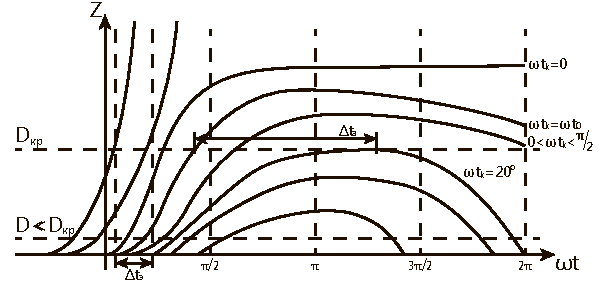
\includegraphics[width=.8\textwidth]{27_Z(wt)} \\
  \caption{Семейство кривых \( Z(\omega t) \)}
  \label{pic27Z(wt)}
\end{figure}

Существовать могут только те электроны, угол влета \( \omega t_k \) которых
лежит в интервале \( [\omega t_0; \pi / 2] \). Остальные же электроны не
покидают катод~-- эмиссия не происходит.

Все электроны, эмитирующиеся с катода, можно условно разделить на три группы в
зависимости от угла влета:
\begin{enumerate}
  \item угол влета \( \omega t_k > 20^\circ \)~-- электроны возвращаются на
    катод в пределах одного периода высокочастотного поля;
  \item угол влета \( \omega t_k \in (0^\circ, 20^\circ) \)~-- электрона при
    движении за период высокочастотного поля поворачивают к катоду, но не
    достигают его.
  \item угол влета \( \omega t_k < 0^\circ \). Эмиссия таких электронов
    возможна, если \( -U_0 > 0 \). Все электроны, эмитируемые с катода,
    движутся к аноду, не меняя своего направления.
\end{enumerate}

Безразмерный параметр \( Z = \alpha z \) называется приведенной координатой.
Тогда параметр \( D = \alpha d \) является приведенным расстоянием катод-анод.
Тогда расстояние \( D_\text{кр} \), которого достигают электроны с углом вылета
\( \omega t_k = 20^\circ \), назовем критическим.

Если \( D \ll D_\text{кр} \), то все электроны будут достигать анода.

Если \( D \gtrsim D_\text{кр} \), то появляется возможность модулировать
эмиссию.
